% Preamble

\documentclass[../main.tex]{subfiles}
\graphicspath{{\subfix{../images/}}}

\begin{document}



\section{Basic concepts}

\subsection{Definition}

According to ITU, telecommunication is any transmission, emission or reception of signs, signals, writings, images and sounds or intelligence of any nature by wire, radio, optical or other electromagnetic systems. Then, a telecommunication system is a bounded technological gadget to provide this service.

\subsection{Characterization}

A telecommunication system can be characterized by the following parameters:

\begin{itemize}
	\item Transmission quality, usually using objective measurements like probability of error ($P_e$) and signal-to-noise ratio ($SNR$), but also using subjective criteria.
	\item Delay in propagation or network access.
	\item Availability in time and location.
\end{itemize}

\subsection{Telecommunication systems architecture}

Telecommunication systems are implemented through networks and terminals.

In order to describe telecommunication systems, we define two elements:

\begin{itemize}
	\item Functional entity: Set of functions in the network with common goal. It might be a physical equipment or not.
	\item Reference points (interfaces): Connections between functional entities.
\end{itemize}

\begin{figure}[H]
	\centering
	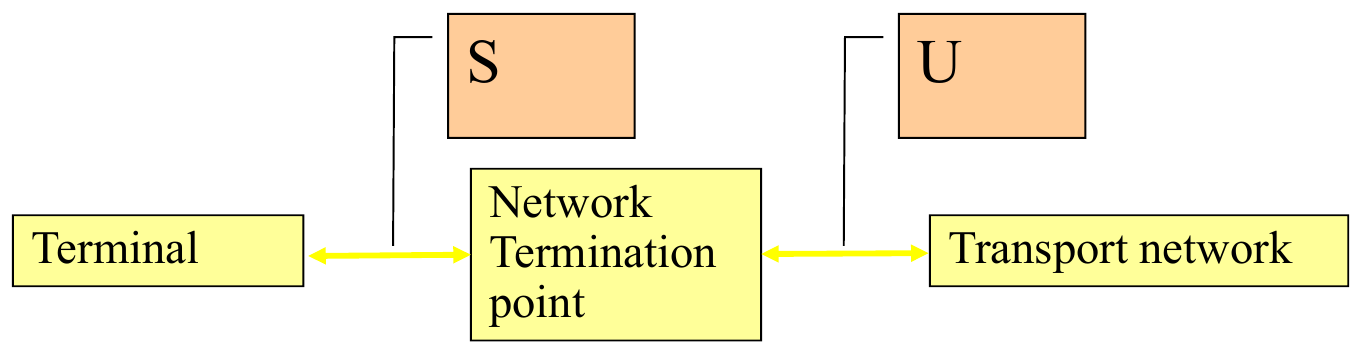
\includegraphics[
		width=14cm,
		%height=15cm
	]{images/Tema 1/Architecture.png}
	\caption{
		\label{fig:unit1_arch}
		Telecommunication systems architecture
	}
\end{figure}

\subsection{Communications networks}

A network is a set of organized resources both logical and physical for allowing the telecommunication. To accomplish with that purpose, the carry out:

\begin{itemize}
	\item Transmission and reception.
	\item Switching.
	\item Signaling.
\end{itemize}

The network is a limited resource and it must be shared, for which networks implement two strategies:

\begin{itemize}
	\item {
		Multiplexing

		\begin{figure}[H]
			\centering
			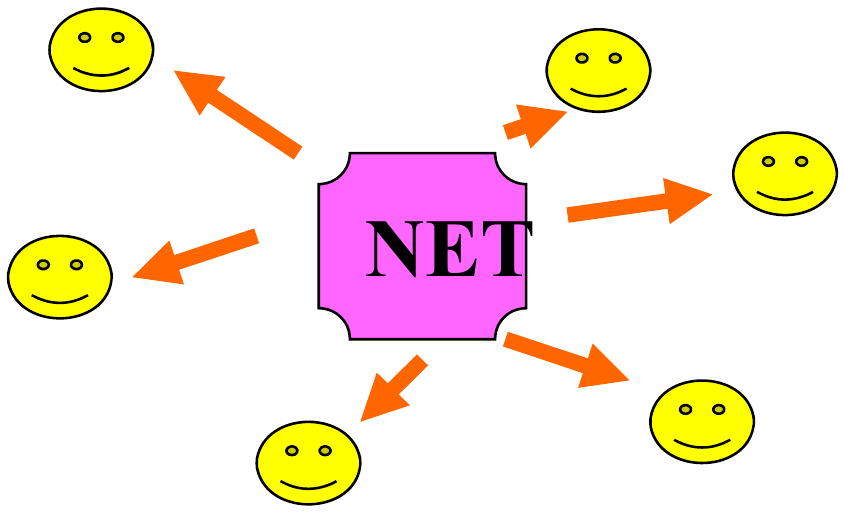
\includegraphics[
				%width=14cm,
				height=3cm
			]{images/Tema 1/Multiplexation.png}
			\caption{
				\label{fig:unit1_muiltiplexation}
				Multiplexing
			}
		\end{figure}
	}
	\item {
		Multiple access

		\begin{figure}[H]
			\centering
			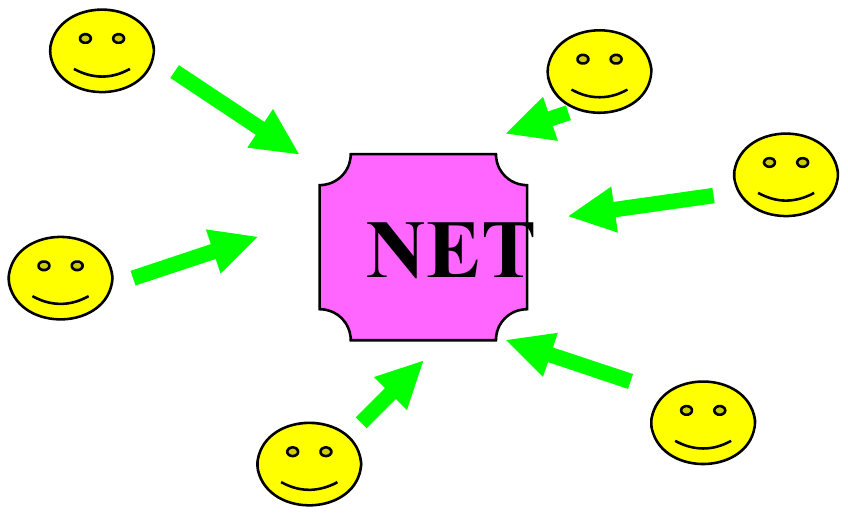
\includegraphics[
				%width=14cm,
				height=3cm
			]{images/Tema 1/Multiple access.png}
			\caption{
				\label{fig:unit1_multiple}
				Multiple access
			}
		\end{figure}
	}
\end{itemize}

Althought many communications networks can perform both broadcasting and switching, due to specialization, they can be classified in these categories:

\begin{itemize}
	\item {
		Broadcast networks: Their purpose is distributing information from a transmitter to a wide number of users, so the transmitter sends the information to the shared medium from which users can access to data. Each terminal selects information addressed to it. Some examples are television network and Local Area Networks (LAN).

		\begin{figure}[H]
			\centering
			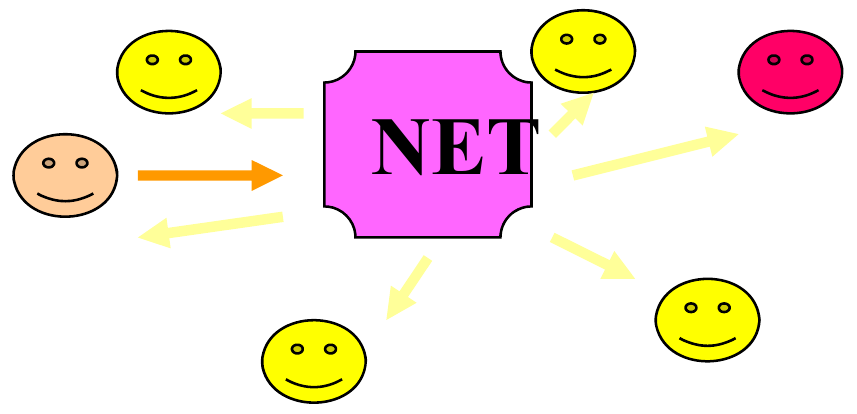
\includegraphics[
				%width=14cm,
				height=3cm
			]{images/Tema 1/Broadcasting.png}
			\caption{
				\label{fig:unit1_broadcast}
				Broadcast networks
			}
		\end{figure}
	}
	\item {
		Switching networks: Their purpose is being specific with source and destination, usually the source terminal selects the destination. The network must establish a physical channel between both terminals. An example is Plain Old Telephony Service (POTS).

		\begin{figure}[H]
			\centering
			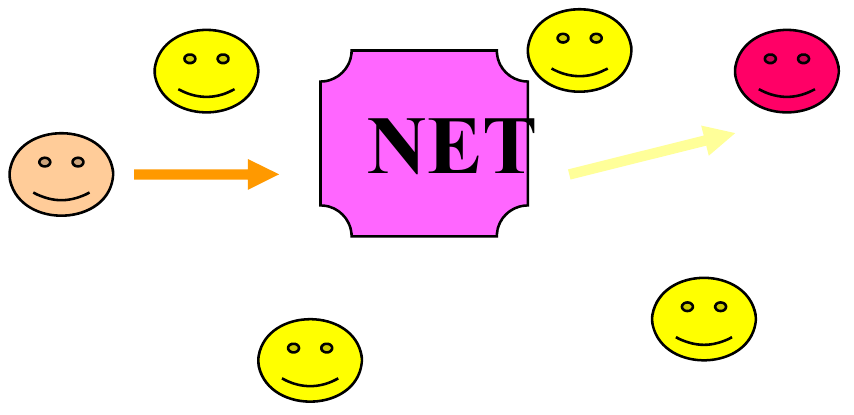
\includegraphics[
				%width=14cm,
				height=3cm
			]{images/Tema 1/Switching.png}
			\caption{
				\label{fig:unit1_switching}
				Switching networks
			}
		\end{figure}
	}
\end{itemize}

\subsection{Telecommunication services}

A service is a set of logical and physical wherewithal operated and managed by the service provider to serve the client and a set of rules for usage and access. All together satisfy the telecommunication required by users.

Services can be classified in many ways:

\begin{itemize}
	\item {
		In function of their complexity:
		\begin{itemize}
			\item Basic services: They exist by their own, like the basic telephony service.
			\item Suplementary services: They are associated to a basic service. Some examples are Calling Line Identification, waiting call, Explicit Call Transfer, Call Hold, multiparty service, etc.
		\end{itemize}
	}
	\item {
		According to ITU:
		\begin{itemize}
			\item Bearer services: They provide the transport capacity.
			\item Teleservices or end services: They provide complete communication capacity. They include terminals even it hey are not provided by the service provider. They include added value services like storage or processing.
		\end{itemize}
		\begin{figure}[H]
			\centering
			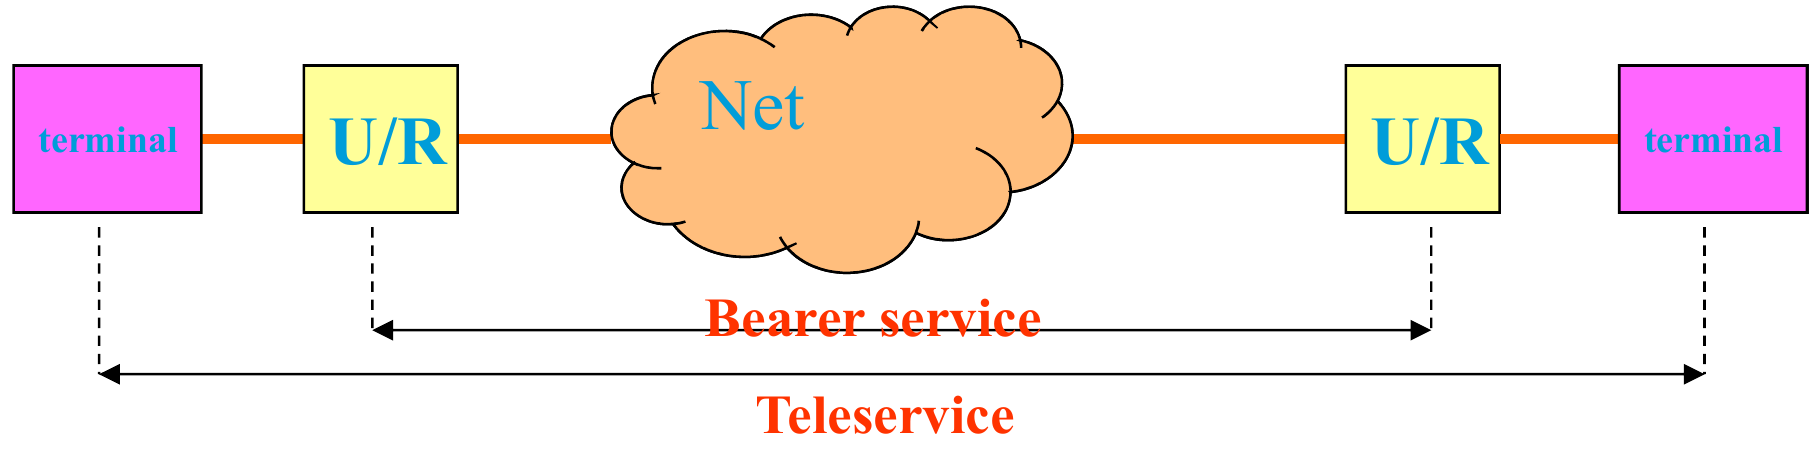
\includegraphics[
				width=14cm,
				%height=15cm
			]{images/Tema 1/Classification according to ITU.png}
			\caption{
				\label{fig:unit1_according}
				Classification according to ITU
			}
		\end{figure}
	}
	\item {
		Other classifications:

		\begin{itemize}
			\item Users' groups: intercommunication, social communications, commercial, residential, ...
			\item Type of information: voice, data, text, control, telemetry, ...
			\item {
				Capacity: wideband, narrowband, ...

				\begin{figure}[H]
					\centering
					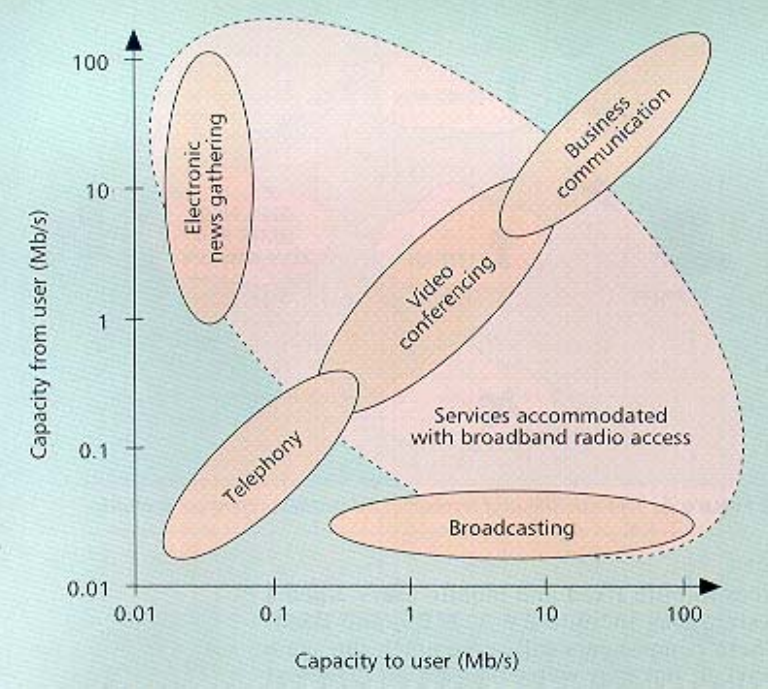
\includegraphics[
						width=14cm,
						%height=15cm
					]{images/Tema 1/Classification in function of capacity.png}
					\caption{
						\label{fig:unit1_capacity}
						Classification in function of capacity
					}
				\end{figure}
			}
			\item Type of communication: query, broadcast, conversation, messages, symmetric, asymmetric, ...
			\item {
				Mobility: fixed, portable, mobile, ...

				\begin{figure}[H]
					\centering
					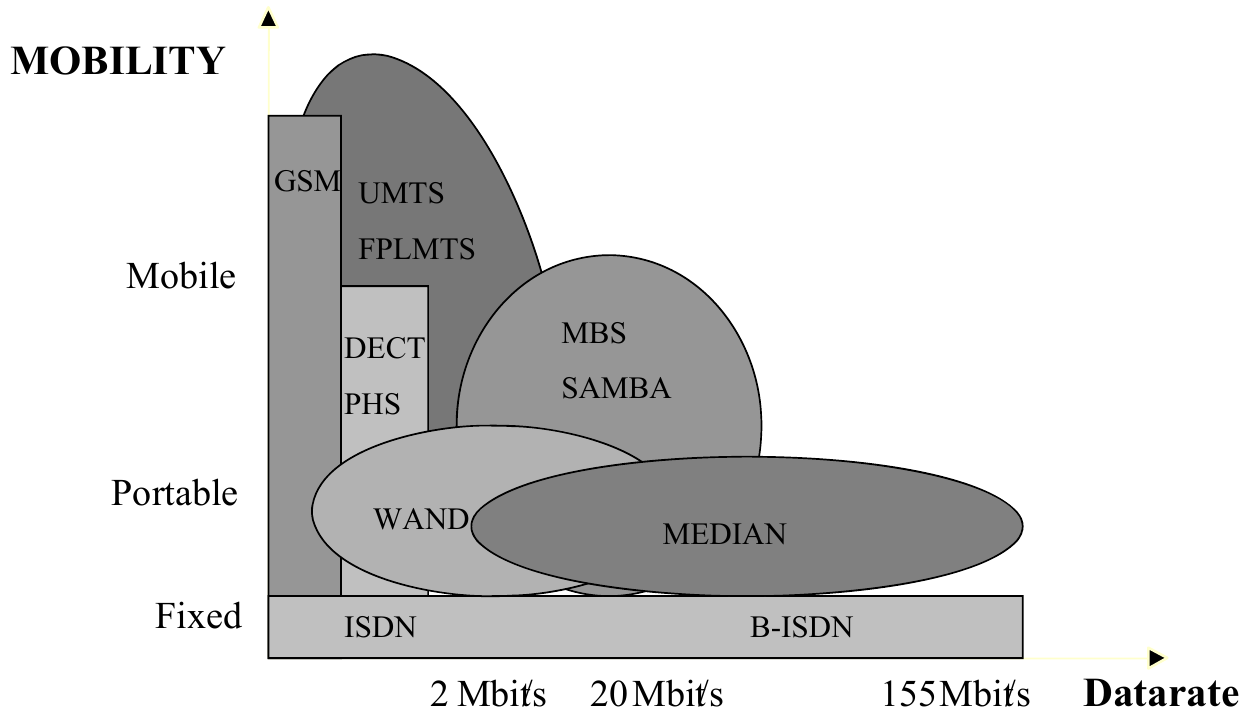
\includegraphics[
						width=13cm,
						%height=15cm
					]{images/Tema 1/Classification in function of mobility.png}
					\caption{
						\label{fig:unit1_mobility}
						Classification in function of mobility
					}
				\end{figure}
			}
			\item Type of network: POTS, ISDN, radio, ...
		\end{itemize}
	}
\end{itemize}

For further study, the main services to consider are:

\begin{itemize}
	\item Telephony service: Their purpose is voice transmission among users. It is high demanded and the most representative. Around it, new services are included, like digitality and mobility, ...
	\item Data transfer service: Their purpose is digital data transmission. It is supported by POTS or specific data networks
	\item Added value services: fax, dataphone, videotex, teletext, ...
	\item Radio communication services: Air is the physical medium to transmit through.
\end{itemize}

\section{Telecommunications regulations}

\subsection{Introduction}

For the propper development of telecommunications, legal and institutional regulations are applied. Their purpose is:

\begin{itemize}
	\item Fair use of electromagnetic spectrum.
	\item Achieve compatibility between telecommunication systems.
	\item Ease the development of economies of scale.
\end{itemize}

\subsection{Spectral regulation}

In wireless communications, electromagnetic spectrum usage must be optimized. This purpose is carried out through the following processes:

\begin{itemize}
	\item Allocation: Entry in a table of frequency allocations of a \textbf{frequency band} for the \textbf{preferent purpose} of its use by one or more terrestrial service, space radiocommunication service or radioastronomy service under specified conditions. This term shall also be applied to the frequency band concerned, which is refered as allocated band.
	\item Allotment: Entry of a designated \textbf{radio frequency or radio frequency channel} in an agreed plan, adopted by a competent conference for its use by one or more administrations for a terrestrial or space radiocommunication \textbf{preferent service} in one or more identified countries or geographical areas and under specified conditions. This term shall also be applied to the radio frequency or radio frequency channel concerned, which is refered as alloted radio frequency or alloted radio frequency channel.
	\item Assignment: \textbf{Authorization given by an administration for a radio station to use a radio frequency or radio frequency channel} under specified conditions. This term shall also be applied to the radio frequency or radio frequency channel concerned, which is refered as assigned radio frequency or assigned radio frequency channel.
\end{itemize}

\subsection{Organizations for the telecommunication regulation}

For the propper development and application of regulations and common standards, there are specific institutions and associations. Main organizations are:

\begin{itemize}
	\item {
		International Telecommunication Union (ITU): Dependant on United Nations. Its purpose is to \textbf{harmonize} the telecommunication \textbf{worldwide} through cooperation, development and normalization. It is divided into temporal committees, but has some permanent bodies:
		\begin{itemize}
			\item Secretary.
			\item UIT-R: Radiocommunications.
			\item UIT-T: Telegraphy, telephony and telematics.
			\item Frequency register.
		\end{itemize}
	}
	\item International Standardization Organization (ISO): It is an international association of national standards organizations. It \textbf{facts norms} \textbf{worldwide}. Some ISO standards examples are: credit card format, telephony cards, intelligent cards, ISO 9000 (quality management).
	\item World Radio Conference (WRC): It defines \textbf{worldwide} \textbf{frequency bands and services}.
	\item Institute of Electrical and Electronic Engineers (IEEE or IE3): It is an independent organization that developes technology standards. It \textbf{facts norms} \textbf{worldwide}.
	\item Federal Communications Commission (FCC): It is an independent agency of United States government. Its purpose is to \textbf{harmonize} telecommunications in \textbf{USA}.
	\item American National Standards Institute (ANSI): It is a private organization. It \textbf{facts norms} in \textbf{USA}.
	\item European Commission (EC): It is the general chair for information society in European Union. It carries out projects and programs. It is composed by a group of senior officers.
	\item \textit{Conférence européenne des administrations des postes et télécommunications} (\textit{CEPT}, in English, European Conference of Postal and Telecommunications Administrations): It is an association of national telecommunication organizations from Europe. Its purpose is to \textbf{harmonize} the telecommunication worldwide (specially in \textbf{Europe}) through cooperation, development and normalization.
	\item European Telecommunication Standards Institute (ETSI): Dependant on CEPT. Its purpose is providing standards on telecommunication systems (it \textbf{facts norms} for \textbf{Europe}).
	\item \textit{Asociación Española de Normalización} (\textit{UNE}, former \textit{AENOR}, in English, Spanish Association of Standardization and Certification): It \textbf{facts norms} in \textbf{Spain}.
	\item \textit{Cuadro Nacional de Atribución de Frecuencias} (\textit{CNAF}, in English, National Table of Frequency Allocations): \textbf{Frequency assignment} in \textbf{Spain}.
\end{itemize}

\begin{table}
	\centering
	\begin{tabular}{lcccc}
		\hline
		~				& Telecommunications	& Standards	& Radiofrequencies	& Others \\
		\hline
		International	& ITU 					& ISO, IEEE	& WRC				& \\
		USA				& FCC					& ANSI		&					& \\
		Europe			& CEPT					& ETSI		&					& EC \\
		Spain			&						& UNE		& CNAF				& \\
		\hline
	\end{tabular}
	\caption{
		\label{tab:unit1_organizations}
		Organizations for the telecommunication regulation
	}
\end{table}

\subsection{Telecommuncations regulation in Spain}

Spain have developed its telecommunication policies through a series of laws and royal decrees:

\begin{itemize}

	\item \textit{Ley 11/1998, de 24 de abril, General de Telecomunicaciones} (in English, \textbf{Law 11/1998}, April 24th, General Law of Telecommunications): Its objective is achieve free competition in telecommunication services, for which it establishes licenses for services.

	\item {
		\textit{Ley 32/2003, de 3 de noviembre, General de Telecomunicaciones} (in English, \textbf{Law 32/2003}, November 3rd, General Law of Telecommunications):
		\begin{itemize}
			\item It derogates the former Law 11/1998.
			\item It includes the evolution of telecommunications since the liberalization according to EU directives.
			\item It was later updated by a Royal Decree (\textit{Real Decreto 424/2005, de 15 de abril, por el que se aprueba el Reglamento sobre las condiciones para la prestación de servicios de comunicaciones electrónicas, el servicio universal y la protección de los usuarios}).
		\end{itemize}
	}

	\item {
		\textit{Ley 9/2014, de 9 de mayo, General de Telecomunicaciones} (in English, \textbf{Law 9/2014}, May 9th, General Law of Telecommunications):
		\begin{itemize}
			\item It derogates the former Law 32/2003.
			\item Its objective is to improve free competition and ease investments.
			\item Some of the main differences with previous law is that it includes structural reforms for easing the deployment of new networks (including flat roof expropriation and other controversial actions) and improving innovative and cheaper services for citizens.
			\item There is established a new interministerial committee for radio frequency and health.
			\item {
				It is guaranteed that:
				\begin{itemize}
					\item By 2017, 100\% of Spanish homes would have broadband internet access at 10 Mbps.
					\item By 2020, 100\% of Spanish homes would have broadband internet access at 30 Mbps and 50\% of them would be higher than 100 Mbps.
				\end{itemize}
			}
		\end{itemize}
	}

	\item {
		\textit{Ley 11/2022, de 28 de junio, General de Telecomunicaciones} (in English, \textbf{Law 11/2022}, June 28th, General Law of Telecommunications):
		\begin{itemize}
			\item It derogates the former Law 9/2014.
			\item It pretends to promote the development of telecommunications engineering, products and equipment.
			\item It pretends to give an impulse to computer telephony integration (CTI) even from urbanism by allowing the administration to deploy and hire networks.
			\item It includes non numbering services (WhatsApp, Facebook, Twitter, Instagram, ...).
			\item It pretends to reduce the impediment for new generation and broadband networks, for which expropriation is still in use.
			\item It increases time for radioelectric licenses.
			\item It reduces the universal service, only allowing fixed service and 10 Mbps.
			\item It pretends to include new users' rights, althought in practice they are the same.
		\end{itemize}
	}
\end{itemize}



\end{document}
